\documentclass{classes/SIT-Report-EN}
\usepackage{tabularx}
\usepackage{graphicx}
\usepackage{adjustbox}
\usepackage{lscape}
\usepackage{longtable}

%%Edit your info Here
\begin{document}
\title{How to Break Enigma Codec}
\titleTH{วิธีถอดรหัสเครื่องอินิกมา}
\degree{Bachelor of Science}
\majorProgramEN{Computer Science}
\academicyear{2024}

\author{Alan Mathison Turing}

\majoradvisor{Asst. Prof. Worarat Krathu, Ph.D.}
\coadvisor{Asst. Prof. Chonlameth Arpnikanondt, Ph.D.}
\committeeOne{Asst. Prof. Praset Kanthamanon, Ph.D.}
\committeeTwo{Asst. Prof. Narongrit Waraporn, Ph.D.}
\committeeThree{Lect. Tuul Triyason, Ph.D}
\academicyear{2024}

%%%%%%%%%%
\maketitle
\frontmatter
\maketitleinner
\makeapproval
% ************************** Thesis Abstract **********************************
\begin{abstract}
\lipsum[1]
\vfill
\begin{flushleft}
\textbf{Keywords :} Enigma / Encryption / Cryptanalytic 
\end{flushleft}
\vfill
\end{abstract} %%Edit your Abstract
\input{pages/acknowledgements} %% %%Edit your Acknowledgement

\tableofcontents
\listoftables
\listoffigures
\input{pages/symbols}
\input{pages/abbreviations}

\mainmatter
%%insert your content
%%% Chapter 1 - Introduction %%%
\chapter{Introduction}

%%% Chapter Introduction %%%
This framework aims  to design and build an integrated system that consists of a centralised data management platform in conjunction with a network of interconnected sensors for the verification of sensors and the identification of anomalies will proceed more quickly as a result of this assembly.

The system makes use of a wide variety of sensors, the most prominent of which are the water level and flow rate sensors. This design was inspire by the infrastructure of the water treatment testbed in the School of Computing at Newcastle University serving as its source of inspiration. These sensors send their readings to an aggregate server (AG), which is implemented as a Raspberry Pi in this case. The primary role of the AG is that of a data collector; after collecting the consolidated data, it is then sent on to the principal server. It is anticipated that, in a more comprehensive real-world scenario, additional aggregate servers will relay data to the primary server, which will ensure that field operations are carried out without any interruptions.

%%% 1.1 Background and Rationale %%%
\section{Background and Rationale}
\lipsum[1]

%%% 1.2 Motivation %%%
\section{Motivation}
\lipsum[1]

%%% 1.3 Research Questions %%%
\section{Research Questions}
The research questions addressed in this study are as follows:
\begin{enumerate}
	\item Aggregate server create secure stream $S$ by encoding with BCH coding which predetermine coding parameter to match with the central server
	\item Aggregate server send reading in plain text along with secure stream to the central server
\end{enumerate}

%%% 1.4 Objectives %%%
\section{Objectives}
The objectives of this research can be summarized as follows:
\begin{enumerate}
	\item Aggregate server create secure stream $S$ by encoding with BCH coding which predetermine coding parameter to match with the central server
	\item Aggregate server send reading in plain text along with secure stream to the central server
	\item central server decode secure stream with plain text. If match, the central server continue to process anomaly detection. If not, it will reject those reading and alert the user for unauthenticated readings.
\end{enumerate}

%%% 1.5 Expected Benefits %%%
\section{Expected Benefits}
According to the objective of this research, we expect two benefits as follow:
\begin{enumerate}
	\item Aggregate server create secure stream $S$ by encoding with BCH coding which predetermine coding parameter to match with the central server
	\item Aggregate server send reading in plain text along with secure stream to the central server
\end{enumerate}

%%% 1.6 Scope of Study %%%
\section{Scope of Study}
\lipsum[1]

%%% 1.7 Thesis Organization %%%
\section{Thesis Organization}
This thesis is divided into five chapters as follows:
\begin{itemize}
	\item Chapter 1 is the introduction of the study. This chapter describes the introduction of the study, explain more.
	\item Chapter 2 presents the literature review of this study. This chapter explains the relevance of models, theories and concepts, explain more.
	\item Chapter 3 proposes the research methodology. This chapter illustrates the research procedures by identifying the step and process of working, explain more.
	\item Chapter 4 describes the results and discussion. This chapter analyzes the data by using some proper statistical data analysis methods, explain more.
	\item Chapter 5 explains the conclusions and future works. This chapter concludes the thesis and future directions of the research, explain more.
\end{itemize}
%%% Chapter 2 - Literature Reviews %%%
\chapter{Literature Reviews}

%%% Chapter Introduction %%%
This framework aims  to design and build an integrated system that consists of a centralised data management platform in conjunction with a network of interconnected sensors for the verification of sensors and the identification of anomalies will proceed more quickly as a result of this assembly.

%%% 2.1 Challenges It Faces Indicating The Need For This Research %%%
\section{Challenges It Faces Indicating The Need For This Research}
\lipsum[1]
\begin{figure}[!h]
	\centering
	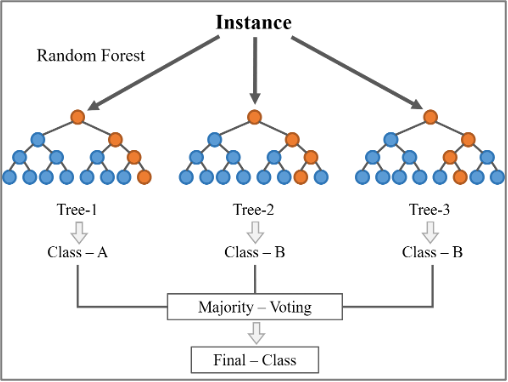
\includegraphics{chapter2/RandomForestClassification.png}
	\caption{Random Forest Classification}
	\label{fig:RandomForestClassification}
\end{figure}

From figure \ref{fig:RandomForestClassification} shows an optimized model that endeavors to heighten detection rates, precision, and processing times \cite{anderson2014engaging}. The innovative architecture integrates the Catboost classifier, melding Gradient Boosting (GB) with Decision Trees (DT). This synergy serves to curtail gradient estimation bias, consequently amplifying the model's generalization prowess. A significant attribute of this model is its utilization of GPU during the training phase, ensuring swifter computations.

	%%% 2.1.1 Fishbone Diagram %%%
	\subsection{Fishbone Diagram}
	\lipsum[1]
	\begin{figure}[!h]
		\centering
		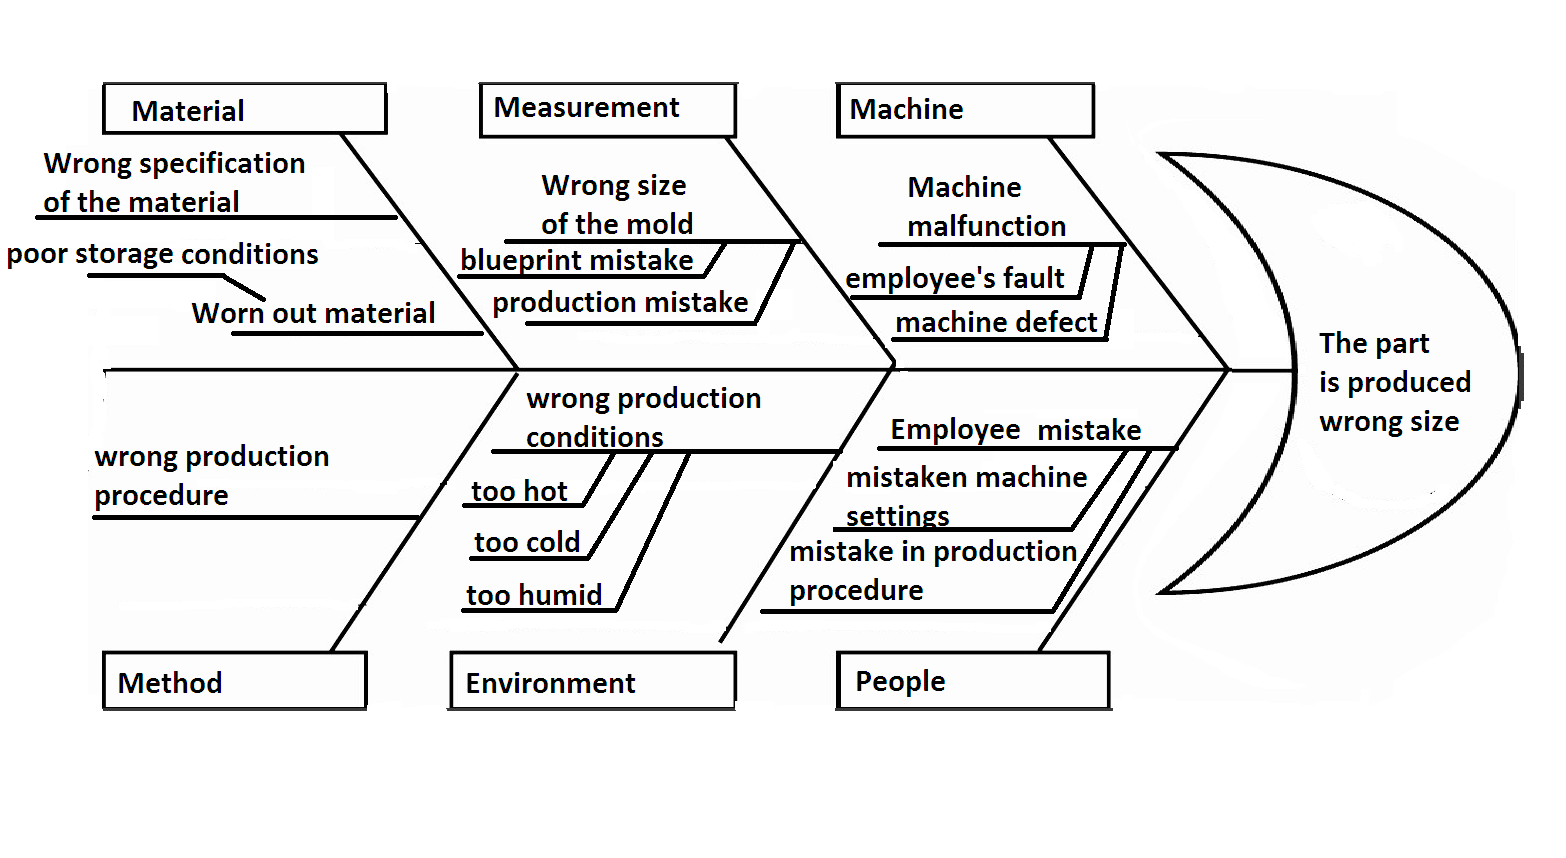
\includegraphics[height=7cm]{chapter2/fishbone.png}
		\caption{Fishbone Diagram}
		\label{fig:FishboneDiagram}
	\end{figure}
	
	From figure \ref{fig:FishboneDiagram} shows an optimized model that endeavors to heighten detection rates, precision, and processing times \cite{anderson2014engaging}. The innovative architecture integrates the Catboost classifier, melding Gradient Boosting (GB) with Decision Trees (DT). This synergy serves to curtail gradient estimation bias, consequently amplifying the model's generalization prowess. A significant attribute of this model is its utilization of GPU during the training phase, ensuring swifter computations.
	
	%%% Add more items depends on your research %%%
	
	%%% 2.1.X Conclusion %%%
	\subsection{Conclusion}
	\lipsum[1]

%%% Chapter 3 - Research Methodology %%%
\chapter{Research Methodology}

%%% Chapter Introduction %%%
This framework aims  to design and build an integrated system that consists of a centralised data management platform in conjunction with a network of interconnected sensors for the verification of sensors and the identification of anomalies will proceed more quickly as a result of this assembly.

%%% 3.1 RQ1 %%%
\section{RQ1: Your Research Question}

%%% 3.1.1 Population and Sample %%%
\subsection{Population and Sample}
\lipsum[1]

Lorem ipsum dolor sit amet, consectetur adipiscing elit. Vivamus a magna a orci lacinia malesuada eget sed odio. Donec et posuere tellus. Etiam fermentum lorem eu imperdiet dictum. Integer consequat dolor sem, id pharetra est vehicula sed. Nam eget feugiat justo.
\begin{enumerate}
	\item Aggregate server create secure stream $S$ by encoding with BCH coding which predetermine coding parameter to match with the central server
	\item Aggregate server send reading in plain text along with secure stream to the central server
	\item central server decode secure stream with plain text. If match, the central server continue to process anomaly detection. If not, it will reject those reading and alert the user for unauthenticated readings.
\end{enumerate}

%%% 3.2 RQ2 %%%
\section{RQ2: Your Research Question}

%%% 3.2.1 Population and Sample %%%
\subsection{Population and Sample}
\lipsum[1]

Lorem ipsum dolor sit amet, consectetur adipiscing elit. Vivamus a magna a orci lacinia malesuada eget sed odio. Donec et posuere tellus. Etiam fermentum lorem eu imperdiet dictum. Integer consequat dolor sem, id pharetra est vehicula sed. Nam eget feugiat justo.
\begin{enumerate}
	\item Aggregate server create secure stream $S$ by encoding with BCH coding which predetermine coding parameter to match with the central server
	\item Aggregate server send reading in plain text along with secure stream to the central server
	\item central server decode secure stream with plain text. If match, the central server continue to process anomaly detection. If not, it will reject those reading and alert the user for unauthenticated readings.
\end{enumerate}

%%% 3.3 RQ3 %%%
\section{RQ3: Your Research Question}

%%% 3.3.1 Population and Sample %%%
\subsection{Population and Sample}
\lipsum[1]

Lorem ipsum dolor sit amet, consectetur adipiscing elit. Vivamus a magna a orci lacinia malesuada eget sed odio. Donec et posuere tellus. Etiam fermentum lorem eu imperdiet dictum. Integer consequat dolor sem, id pharetra est vehicula sed. Nam eget feugiat justo.
\begin{enumerate}
	\item Aggregate server create secure stream $S$ by encoding with BCH coding which predetermine coding parameter to match with the central server
	\item Aggregate server send reading in plain text along with secure stream to the central server
	\item central server decode secure stream with plain text. If match, the central server continue to process anomaly detection. If not, it will reject those reading and alert the user for unauthenticated readings.
\end{enumerate}
%%% Chapter 4 - Results and Discussion %%%
\chapter{Results and Discussion}

%%% Chapter Introduction %%%
This framework aims  to design and build an integrated system that consists of a centralised data management platform in conjunction with a network of interconnected sensors for the verification of sensors and the identification of anomalies will proceed more quickly as a result of this assembly.

%%% 4.1 Modeling Results %%%
\section{Modeling Results}
\lipsum[1-3]
%%% Chapter 5 - Conclusions %%%
\chapter{Conclusions}

%%% Chapter Introduction %%%
This framework aims  to design and build an integrated system that consists of a centralised data management platform in conjunction with a network of interconnected sensors for the verification of sensors and the identification of anomalies will proceed more quickly as a result of this assembly.

%%% 5.1 Summary %%%
\section{Summary}
\lipsum[1-3]

%%% 5.2 Contributions %%%
\section{Contributions}
\lipsum[1-3]

%%% 5.3 Future Works %%%
\section{Future Works}
\lipsum[1-3]


\bibliographystyle{plain}
\bibliography{references/references}
\addcontentsline{toc}{chapter}{REFERRENCES}

\begin{appendices}
	\input{appendix/appendix1}
\end{appendices}

\end{document}
